\chapter{精修：直接求导并消除无效自由度}
\section{目标函数与物理参数}
对已校正、可视为独立的带符号强度，原生精修最小化
\begin{equation}
 Q(\theta)=\sum_{h\in\mathcal W}w_h[y_h-I_h(\theta)]^2
             +\sum_m r_m(\theta)^2.
\end{equation}
第一项使用工作集，第二项是明确给出的结构限制。$w_h=1/\sigma_h^2$ 是基本选择。保留的经验权重模式使用外层冻结权重迭代；每次最小二乘只对这一轮固定的权重求导，并记录权重是否达到固定点。训练使用全部有效 $F^2$，$I>2\sigma(I)$ 只出现在传统 $R_1$ 指标的定义里\cite{shelxl2015}。

\section{解析导数的来源}
令原子某一对称位置的贡献为 $C_{joh}$。对任意独立实参数 $p$，
\begin{align}
 \partial_p C_{joh}
 &=C_{joh}\left(2\pi\iu h^{\mathsf T}\partial_p x_{jo}
      -2\pi^2q^{\mathsf T}(\partial_pU_{jo})q\right)
      +\text{占有率的贡献},\\
 \partial_p|F_h|^2&=2\operatorname{Re}(F_h^*\partial_pF_h).
\end{align}
占有率为零时，不能用 $C/o_j$ 这种形式求导；应直接保留不含占有率的原子贡献。新实现按这一点处理边界。强度尺度 $k$、晶畴比例和对称操作的导数再用链式法则组合。

原实现对每个参数作两次扰动，再重算整张衍射表。新实现只计算一遍当前原子贡献，再累积所有非零切向导数。原子散射因子、固定倒易几何和位置轨道提前缓存；反射按块计算，减少同时存放的复数数组。

\section{正定位移参数与矩阵指数}
各向同性位移参数写为 $u=e^v$，其导数为 $\dif u=u\dif v$。一般位置的各向异性张量用 Cholesky 形式：
\begin{equation}
 U=LL^{\mathsf T},\qquad L_{ii}=e^{v_i},\qquad
 \dif U=(\dif L)L^{\mathsf T}+L(\dif L)^{\mathsf T}.
\end{equation}
这样每次迭代都满足正定性，而不是先得到负特征值再裁切。

特殊位置还要求 $U$ 位于对称性不变的子空间。代码在相应的对称矩阵空间中写 $U=\exp S$。若 $S=Q\diag(s_i)Q^{\mathsf T}$，矩阵指数的 Fréchet 导数为
\begin{equation}
 D\exp(S)[E]=Q\left[K\odot(Q^{\mathsf T}EQ)\right]Q^{\mathsf T},\qquad
 K_{ij}=\begin{cases}
 \dfrac{e^{s_i}-e^{s_j}}{s_i-s_j},&s_i\ne s_j,\\e^{s_i},&s_i=s_j.
 \end{cases}
\end{equation}
重复特征值并不使导数不存在。数值上用 $e^{(s_i+s_j)/2}\operatorname{sinhc}[(s_i-s_j)/2]$ 求这个连续商，避免对不稳定的特征向量进行差分。

\section{比例约束与尺度规范}
晶畴比例和一组和固定的占有率可以用 softmax 表示，固定参考 logit 为零：
\begin{equation}
 \alpha_d=\frac{e^{v_d}}{\sum_ce^{v_c}},\qquad
 \frac{\partial\alpha_d}{\partial v_c}=\alpha_d(\delta_{dc}-\alpha_c).
\end{equation}
固定参考值消除了所有 logit 同时加常数的冗余。它仍不能消除物理模型本身的退化。例如把所有占有率乘 $c$、把强度尺度除以 $c^2$，可能保留相同的计算强度。因此至少需要一个占有率锚点或精确的组成和约束。

P1 中整体平移原子坐标也不改变强度。连续原点自由度应通过明确的规范消去。空间群中的特殊位置多重度是离散选择，不能在连续优化末尾悄然改变；新代码检查这种变化，要求重新声明位置模型。

\section{不通过大矩阵估计信息}
残差的线性化为 $r(\theta+\delta)\approx r+J\delta$。若 $J$ 有零空间，沿相应方向改变参数不会一阶改变观测。代码不再构造完整的观测维左奇异矩阵，而是按块累积
\begin{equation}
 R_{t+1}=\operatorname{qr}_R\begin{bmatrix}R_t\\J_{t+1}\end{bmatrix},
 \qquad R=U_R\Sigma V^{\mathsf T}.
\end{equation}
正交变换保留奇异值，所以可用小矩阵的 $\Sigma,V$ 判断参数秩。条件协方差只在可辨识且处于常规内部的参数上有通常解释：
\begin{equation}
 C_\theta=V\Sigma^{-2}V^{\mathsf T},\qquad
 C_p=G C_\theta G^{\mathsf T},\quad G=\partial p/\partial\theta.
\end{equation}
秩不足时返回零空间和可估计子空间的伪逆；不把伪逆的对角线当作不可辨识参数的真实标准差。受边界影响的标准差同样标明适用范围。报告还分别给出仅由衍射提供的秩和加入限制后的秩。

新的复杂临时数组按反射块大小增长；当前 SciPy 信赖域求解器仍保存实数 $N\times p$ Jacobian，所以不能说整个精修过程只用常数内存。下一步可以在同一导数接口上实现矩阵自由的 $Jv$、$J^{\mathsf T}v$ 和迭代线性求解；本版没有把这项计划写成已实现功能。
\begin{figure}[!htbp]
\centering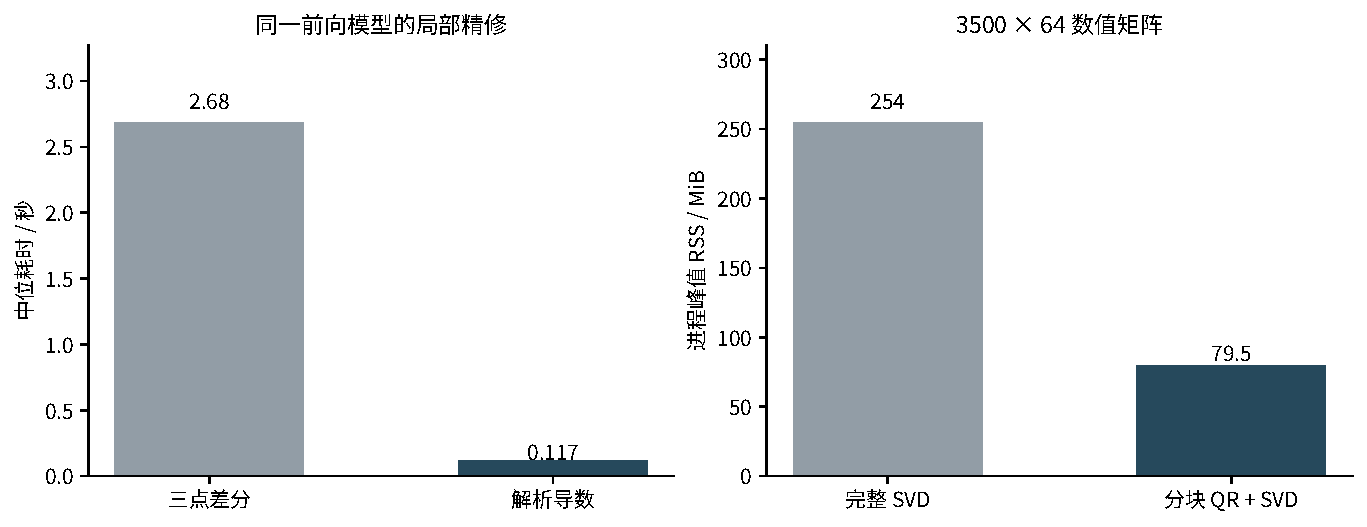
\includegraphics[width=\textwidth]{figures/07_refinement_performance.pdf}
\caption{本次环境中的局部数值基准。左：18 原子、1,098 反射、70 参数的三次单线程中位时间；两条路径使用同一缓存前向模型。右：3500\,$\times$\,64 矩阵的独立进程峰值 RSS，包含解释器和库开销。它们不是与 SHELXL 的速度比较。}\label{fig:performance}
\end{figure}
